\documentclass[a4paper,11pt]{article}
\usepackage[a4paper,total={18cm, 24cm}]{geometry}
\usepackage[parfill]{parskip}
\usepackage[utf8]{inputenc}
\usepackage[T1]{fontenc}
\usepackage{fancyhdr}
\usepackage[ddmmyyyy]{datetime}
\usepackage{graphicx}
\usepackage{subcaption}
\usepackage{multirow}

\pagestyle{fancy}
\fancyhf{}
\lhead{\today}
\chead{Deep Learning - Backpropagation}
\rhead{Jakub Rada}

\begin{document}
\section{Part 1: Tensor basics}
In this part of the assignment we go through some basics of pytorch \texttt{tensors} and computing gradients.
The code is provided in a file \texttt{tensor\_task.py}, this report contains answers to questions and drawings of computation graphs.

\paragraph{(2)} Draw the computation graph for the used expression.
\begin{figure}[ht]
    \centering
    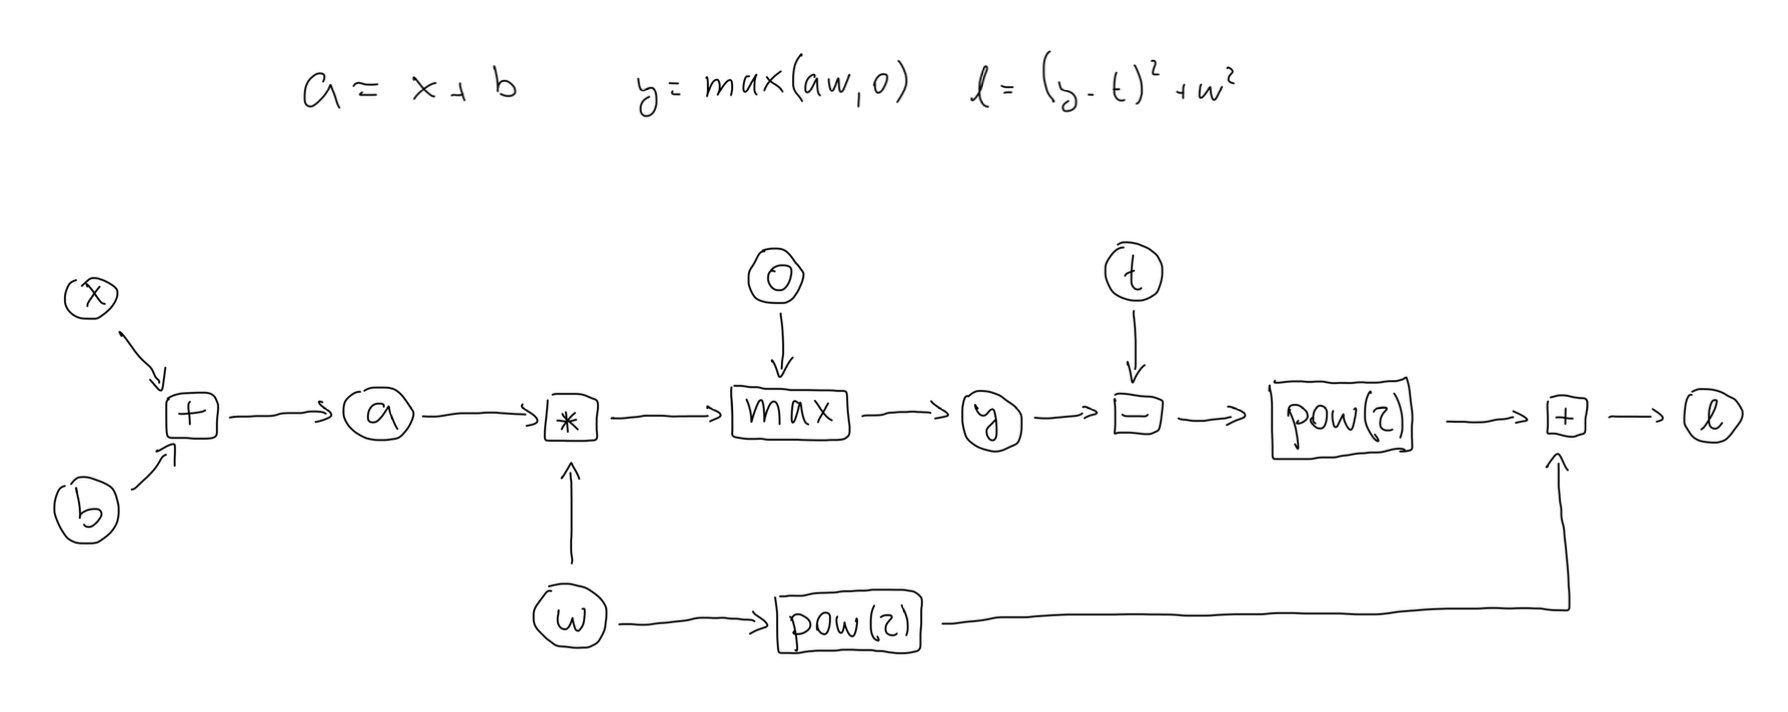
\includegraphics[width=0.8\textwidth]{./DAG.png}
\end{figure}

\texttt{graph\_fn} attributes are as follows:
\begin{table}[ht]
    \centering
    \begin{tabular}{r | l}
        variable & \texttt{graph\_fn}    \\
        y        & \texttt{MulBackward0} \\
        l        & \texttt{AddBackward0} \\
        a        & \texttt{None}         \\
    \end{tabular}
\end{table}

\paragraph{(3)} Derivative of $l$ w.r.t. $y$ is $6.0$.

\paragraph{(4)} Derivative of $l$ w.r.t. $w$ is $38.0$.

\paragraph{(5)} The new value of $w^{\prime} = w - 0.1\nabla_{w}l = -2.799999952316284$.
We need to access the \texttt{.data} attribute because if we added it to the whole tensor, PyTorch would save this update to the computation graph and future backgpropagation could depend also on this computation instead of just the forward pass.
This would lead to wrong results.

\paragraph{(6)} The gradient will be computed correctly, because references to the used tensors are stored in the computation graph, so the garbage collector will not remove them when leaving the scope of the function.
It will remove only the references bound to the variable names.
Also, the \texttt{del} is redundant because the variable references will be removed automatically when the program leaves the scope of the function.

The commented \texttt{y /= 2} causes an error because we try to modify an inner node of the computation graph after it was already used in the forward pass.
This would either lead to inconsistent values of the tensors in the graph or all computations following y in the graph would have to be recomputed again, which does not make sense.

\section{Part 2: Gradient and Network Training}
In the first task, I implemented a neural network as described on the website.
Weights $W_1$, $b_1$, $w$, and $b$ are initialized uniformly at random from interval $[-1, 1]$.

Second task was to check the gradients by comparing the autograd derivative given by backward pass and numerical differentiation by randomly perturbing the weights.
Another goal was to examine the effect of float precision on the outcomes.
I tried values $\epsilon \in \{10^{-2}, 10^{-3}, 10^{-4}, 10^{-5}\}$ for two precisions \texttt{float32} and \texttt{float64}.

The results are following:

\begin{table}[ht]
    \centering
    \begin{tabular}{ r | c | l | l | l | l }
                                          & parameter & $\epsilon = 10^{-2}$ & $\epsilon = 10^{-3}$ & $\epsilon = 10^{-4}$ & $\epsilon = 10^{-5}$ \\
        \hline
        \multirow{4}{*}{\texttt{float32}} & $W_1$     & 1.561e-06            & 1.229e-05            & 0.0001665            & 0.001239             \\
                                          & $b_1$     & 1.706e-06            & 3.747e-05            & 0.0001448            & 0.0003832            \\
                                          & $w$       & 4.023e-07            & 1.982e-06            & 2.582e-05            & 0.000145             \\
                                          & $b$       & 7.153e-06            & 1.907e-05            & 0.0002908            & 0.003166             \\
        \hline
        \multirow{4}{*}{\texttt{float64}} & $W_1$     & 5.04e-06             & 5.039e-08            & 5.043e-10            & 6.063e-12            \\
                                          & $b_1$     & 3.591e-07            & 3.591e-09            & 3.618e-11            & 2.095e-12            \\
                                          & $w$       & 8.944e-07            & 8.948e-09            & 8.943e-11            & 7.229e-13            \\
                                          & $b$       & 3.651e-05            & 3.651e-07            & 3.651e-09            & 3.814e-11            \\
    \end{tabular}
\end{table}

We can see from these numbers that the precision of \texttt{float32} starts to be a problem even for $\epsilon = 10^{-3}$ as the difference between autograd and numerical gradient gets bigger with smaller perturbation.
For even smaller values it only gets worse.
On the other hand, \texttt{float64} confirms the expected precision of the gradient which corresponds to $O(\epsilon^2)$ up to a constant.

In the last task, I trained the network by gradient descent.
I used the suggested values: learning rate $\epsilon = 0.1$, number of epochs $N = 1000$ and size of training data set $M = 200$.
I varied both the activation function, which was either $tanh$ or $ReLU$, and the number of hidden units which was $d \in \{5, 10, 100, 500\}$.

After learning the parameters on the training set I drew a test set and evaluated the test error and generalization gap.
I computed the generalization gap as absolute value of the difference between the training error and test error.
The size of the test set was computed from \textit{Hoeffding inequality} such that the probability of being off the estimate by more than $1\%$ was less than $0.01$.
The size of the test set I derived was rougly $26000$ samples, which I rounded to $30000$ for simplicity in the code.
The derivation is show here:
\begin{figure}[ht]
    \centering
    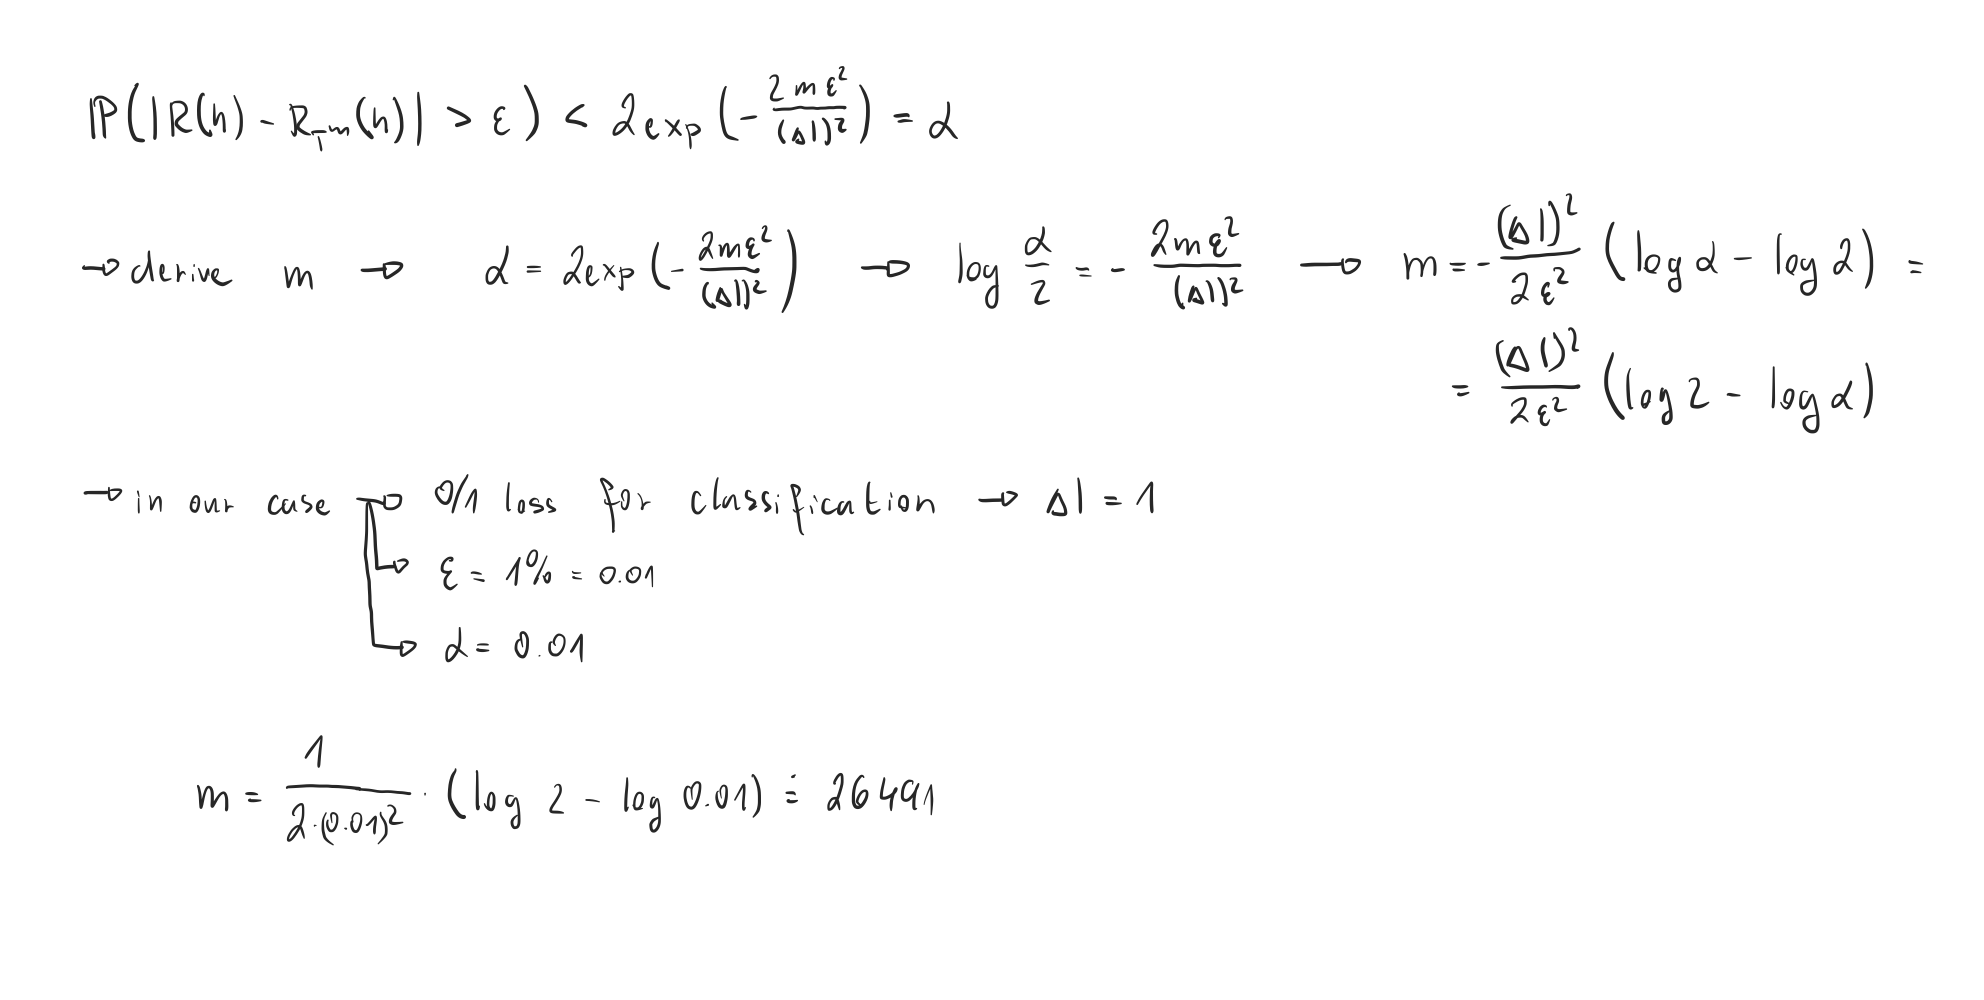
\includegraphics[width=0.7\textwidth]{hoeffding_test_size.png}
\end{figure}

\newpage

The resulting values are shown in the following table:
\begin{table}[ht]
    \centering
    \begin{tabular}{ r | r | c | c }
        activation & hidden units & test error & generalization gap \\
        \hline
        $tanh$     & 5            & 0.0377     & 0.0027             \\
        $tanh$     & 100          & 0.0344     & 0.0044             \\
        $tanh$     & 500          & 0.0281     & 0.0131             \\
        $ReLU$     & 5            & 0.1954     & 0.0504             \\
        $ReLU$     & 100          & 0.0285     & 0.0085             \\
        $ReLU$     & 500          & 0.0216     & 0.0166             \\
    \end{tabular}
\end{table}

Now I show the boundaries of both activations for different number of hidden units.
\begin{figure}[ht]
    \begin{subfigure}[b]{0.3\textwidth}
        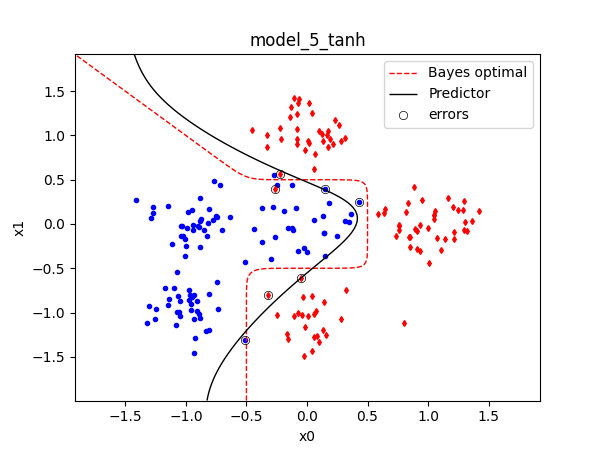
\includegraphics[width=\textwidth]{../boundaries/model_5_tanh.png}
    \end{subfigure}
    \hfill
    \begin{subfigure}[b]{0.3\textwidth}
        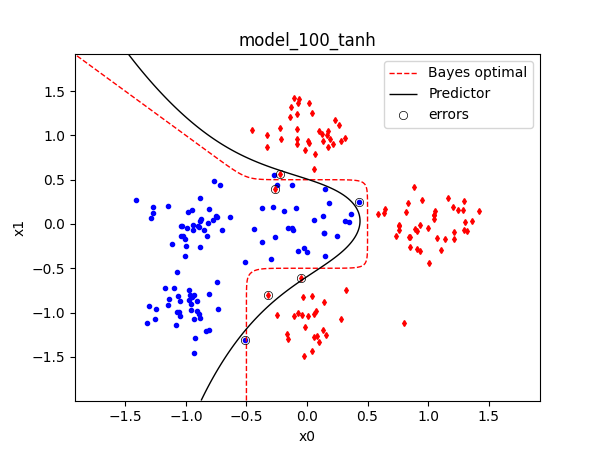
\includegraphics[width=\textwidth]{../boundaries/model_100_tanh.png}
    \end{subfigure}
    \hfill
    \begin{subfigure}[b]{0.3\textwidth}
        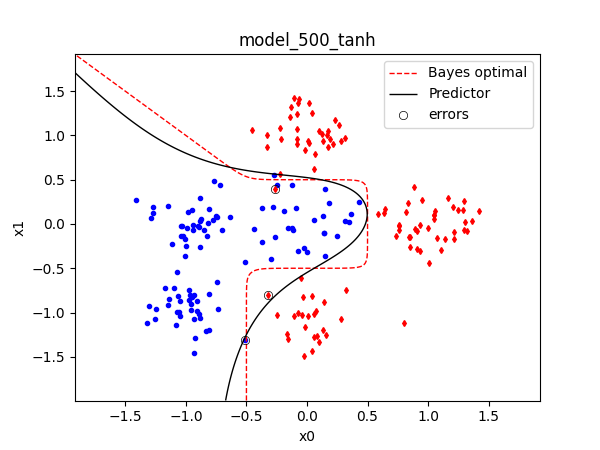
\includegraphics[width=\textwidth]{../boundaries/model_500_tanh.png}
    \end{subfigure}
    \begin{subfigure}[b]{0.3\textwidth}
        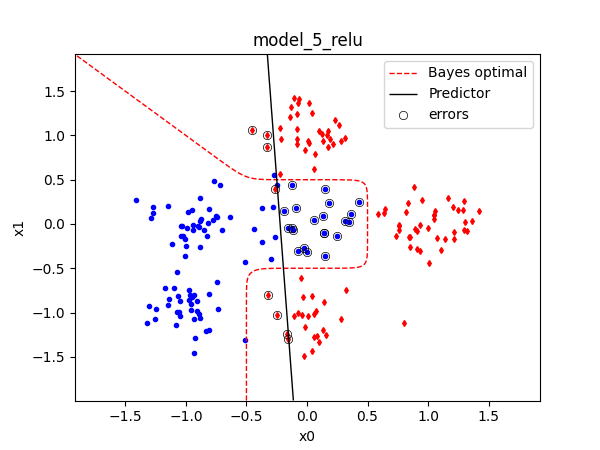
\includegraphics[width=\textwidth]{../boundaries/model_5_relu.png}
    \end{subfigure}
    \hfill
    \begin{subfigure}[b]{0.3\textwidth}
        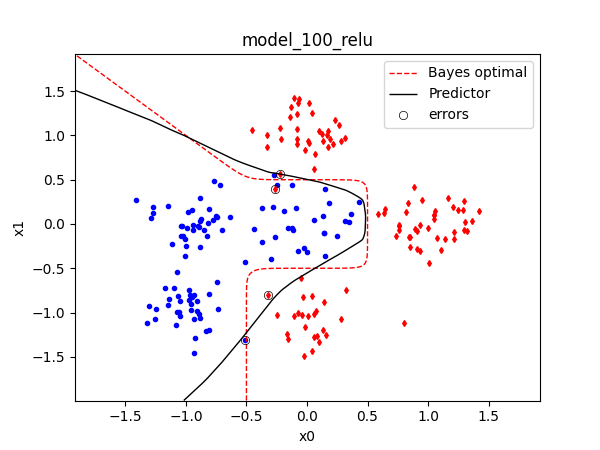
\includegraphics[width=\textwidth]{../boundaries/model_100_relu.png}
    \end{subfigure}
    \hfill
    \begin{subfigure}[b]{0.3\textwidth}
        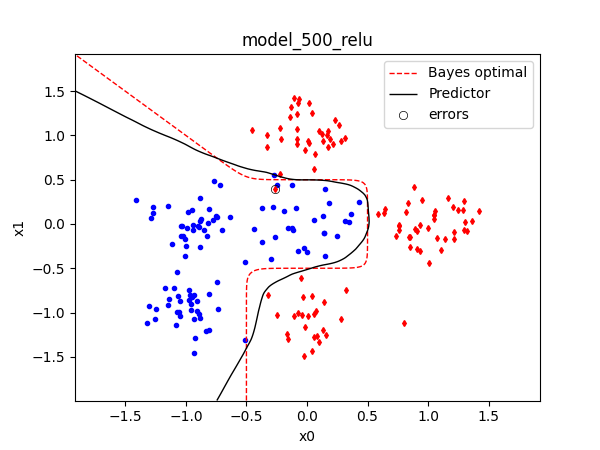
\includegraphics[width=\textwidth]{../boundaries/model_500_relu.png}
    \end{subfigure}
\end{figure}

From these plots we can confirm the hypothesis that the classifier achieves better performance but the decision boundary stays smooth.
Interesting is the case of $ReLU$ with $5$ hidden units, where the decision boundary is almost linear and classifies many points wrong.
But with $100$ and $500$ hidden units, the decision boundary gets much better and even visually outperform the $tanh$ activation.

\section{Part 3: Test Error}
In this last part, we focus on the evaluation of the classifier on the test set.
First, we try to estimate the distribution of the errors by sampling the test set many times and evaluating the classifier on these sample sets.
Then, we compare it to repeated sampling with repetition of a single test set becuase in real-world applications we do not have the possibility to generate many test sets.
To simulate multiple test set sampling we use bootstrapping.
On these data, we compute the confidence intervals according to \textit{Hoeffding inequality}, \textit{Chebyshev inequality}, \textit{Bootstrap} and \textit{Bernstein inequality}.

First, I show the derivations of computing the confidence intervals $R_T \pm \epsilon$ for the three inequalities given confidence level $\alpha = 0.9$ and the size of the test set $m = 1000$.
I derive the computation generaly, numeric computation is only in the code.
\begin{figure}[ht]
    \centering
    \begin{subfigure}[b]{0.45\textwidth}
        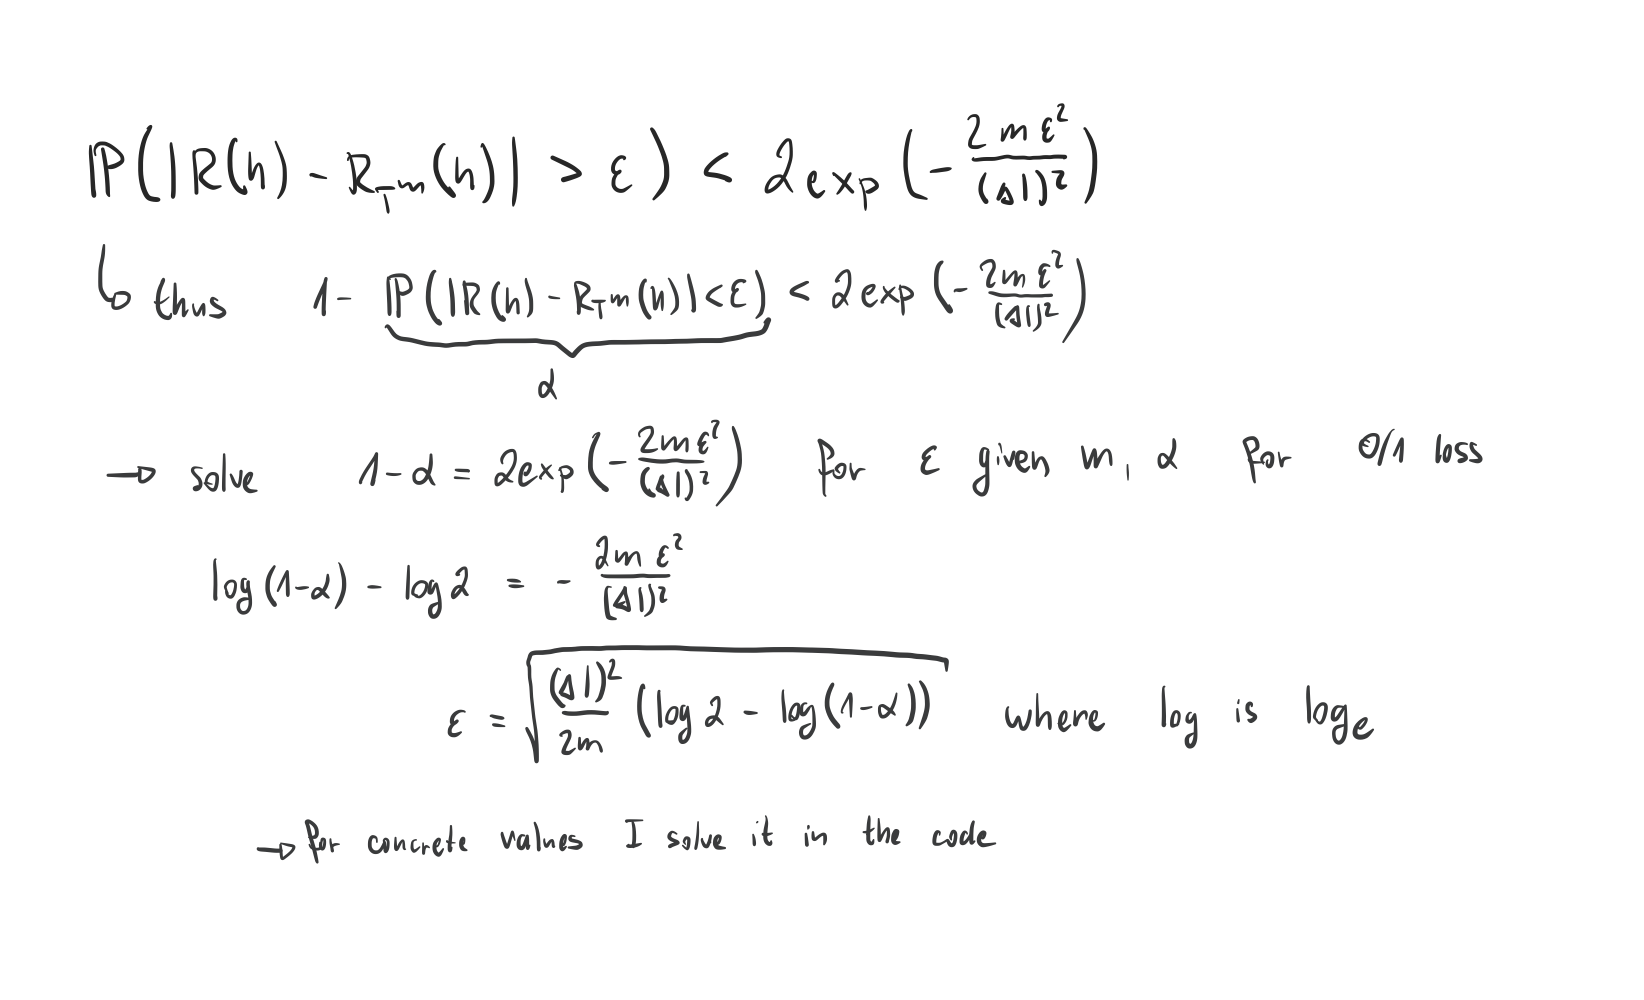
\includegraphics[width=\textwidth]{./hoeffding.png}
        \caption*{Hoeffding inequality}
    \end{subfigure}
    \hfill
    \begin{subfigure}[b]{0.45\textwidth}
        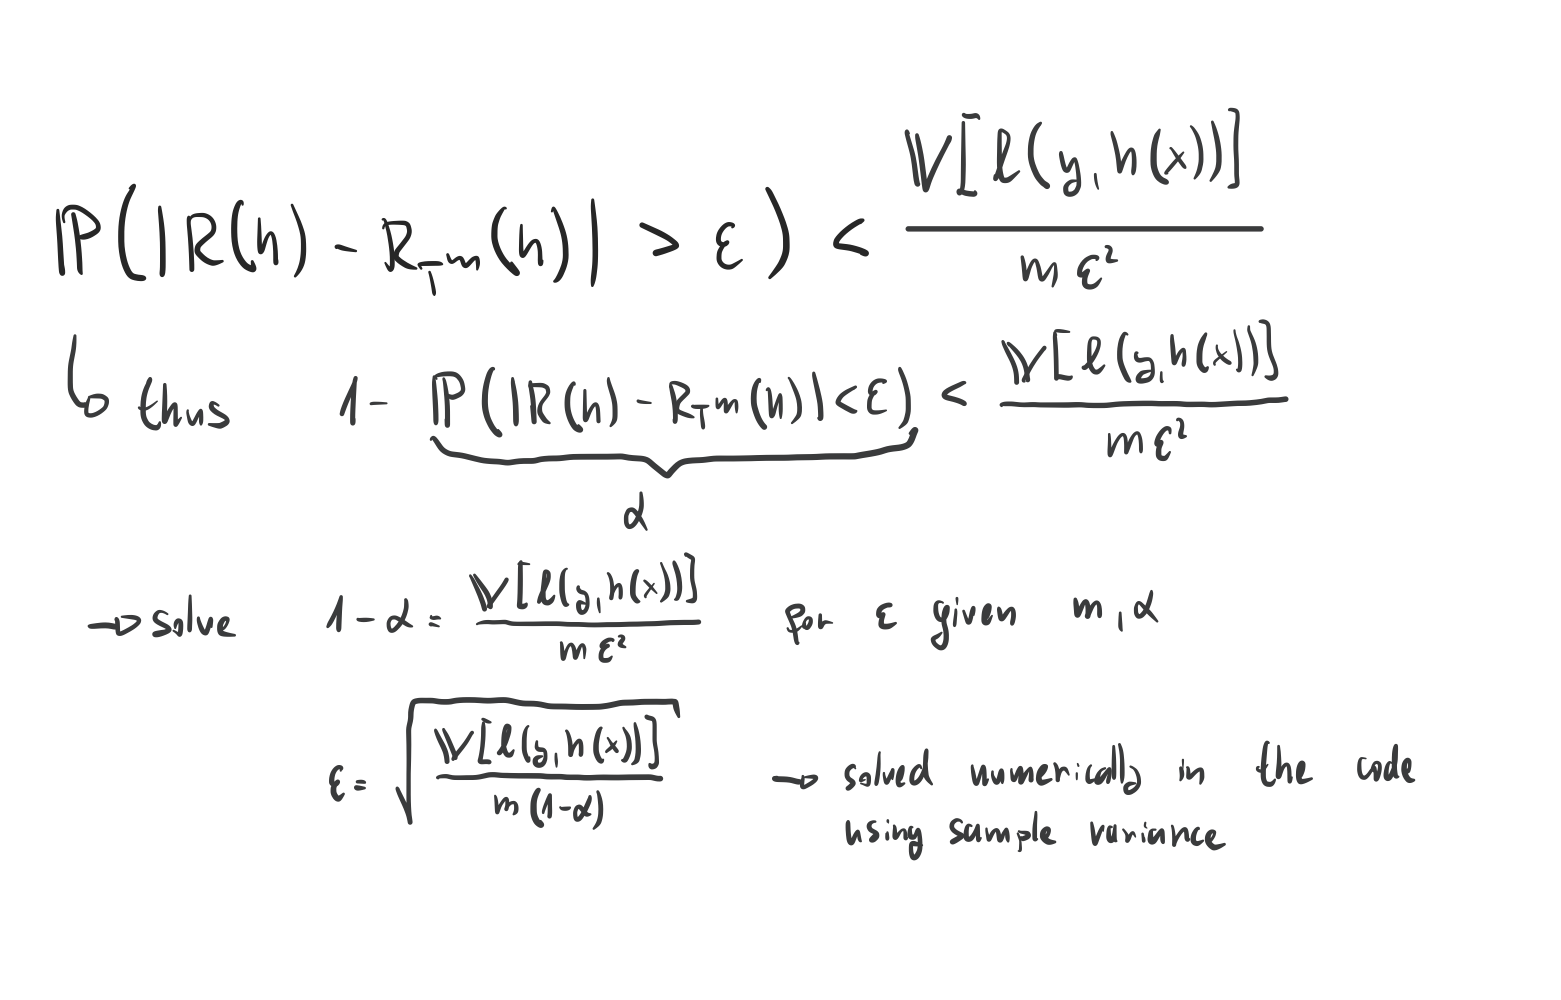
\includegraphics[width=\textwidth]{./chebyshev.png}
        \caption*{Chebyshev inequality}
    \end{subfigure}
    \begin{subfigure}[b]{0.9\textwidth}
        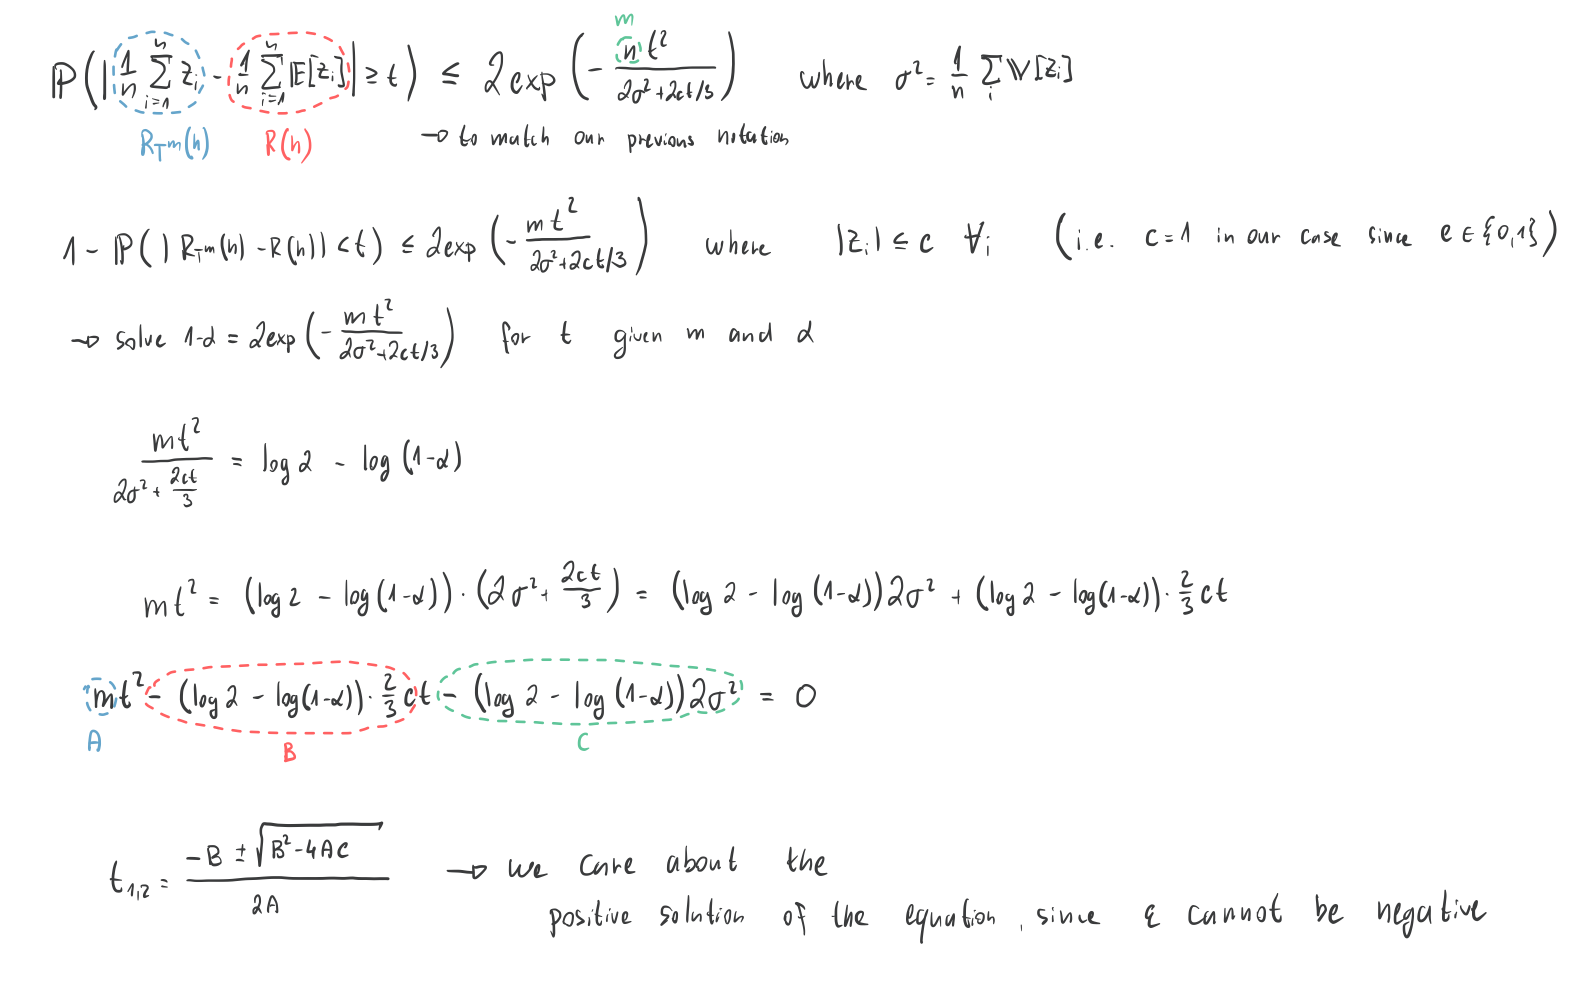
\includegraphics[width=\textwidth]{./bernstein.png}
        \caption*{Bernstein inequality}
    \end{subfigure}
\end{figure}

\newpage

Then, I can show the resulting plots for the activations and numbers of hidden units as in the previous task together with the values of confidence intervals.
\begin{figure}[ht]
    \centering
    \begin{subfigure}[b]{0.45\textwidth}
        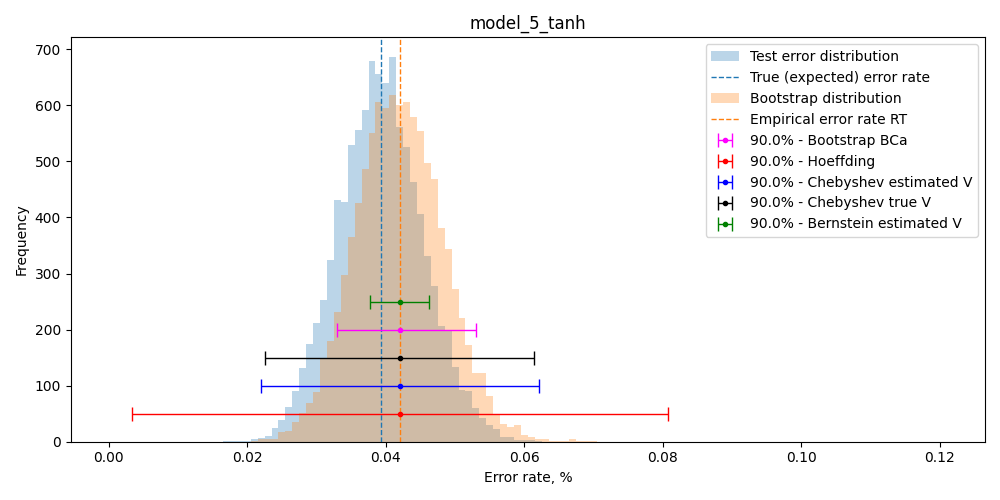
\includegraphics[width=\textwidth]{../errors/model_5_tanh.png}
    \end{subfigure}
    \hfill
    \begin{subfigure}[b]{0.45\textwidth}
        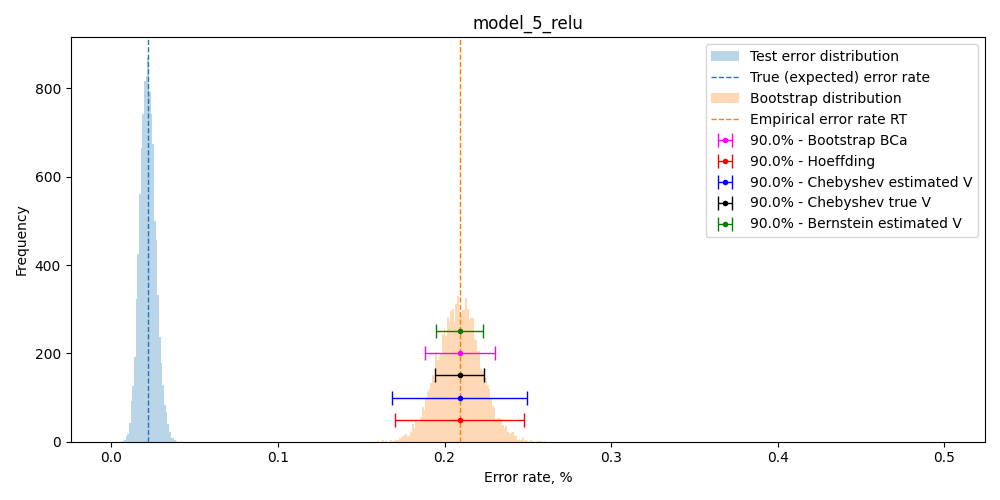
\includegraphics[width=\textwidth]{../errors/model_5_relu.png}
    \end{subfigure}
    \begin{subfigure}[b]{0.45\textwidth}
        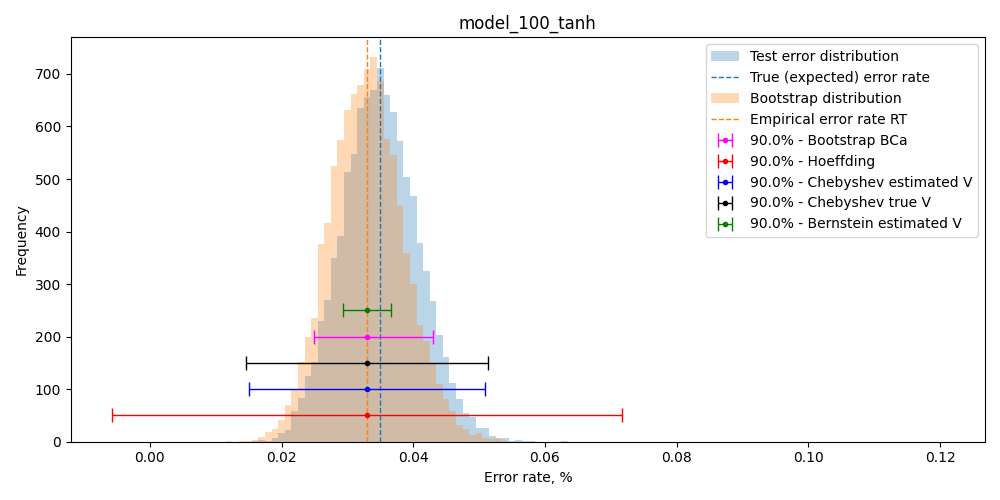
\includegraphics[width=\textwidth]{../errors/model_100_tanh.png}
    \end{subfigure}
    \hfill
    \begin{subfigure}[b]{0.45\textwidth}
        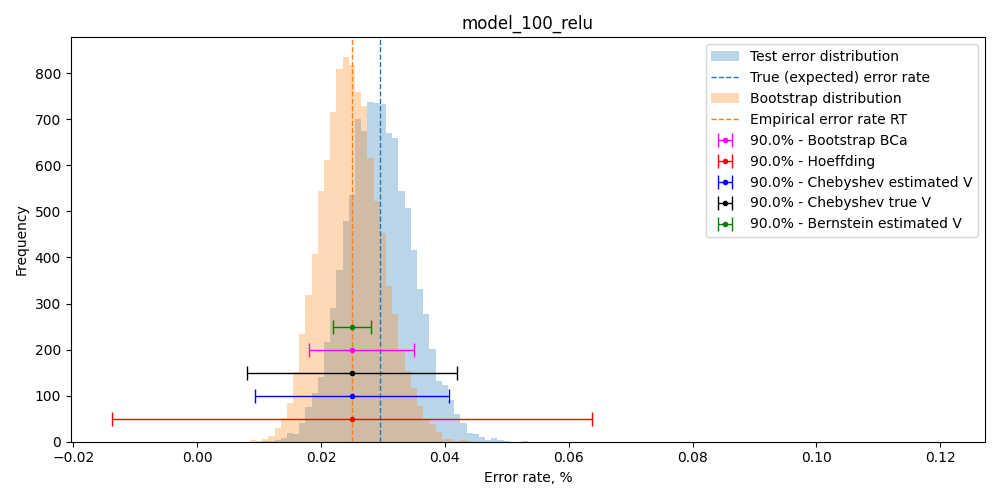
\includegraphics[width=\textwidth]{../errors/model_100_relu.png}
    \end{subfigure}
    \begin{subfigure}[b]{0.45\textwidth}
        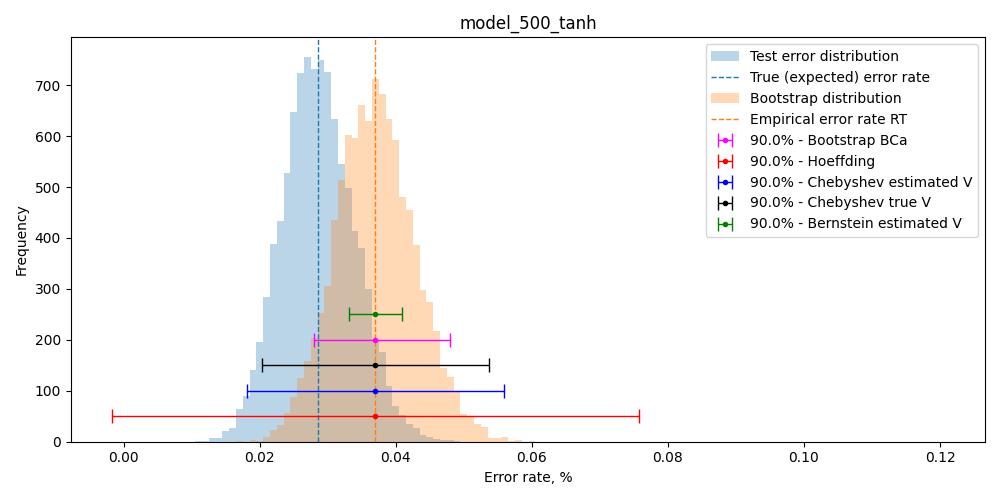
\includegraphics[width=\textwidth]{../errors/model_500_tanh.png}
    \end{subfigure}
    \hfill
    \begin{subfigure}[b]{0.45\textwidth}
        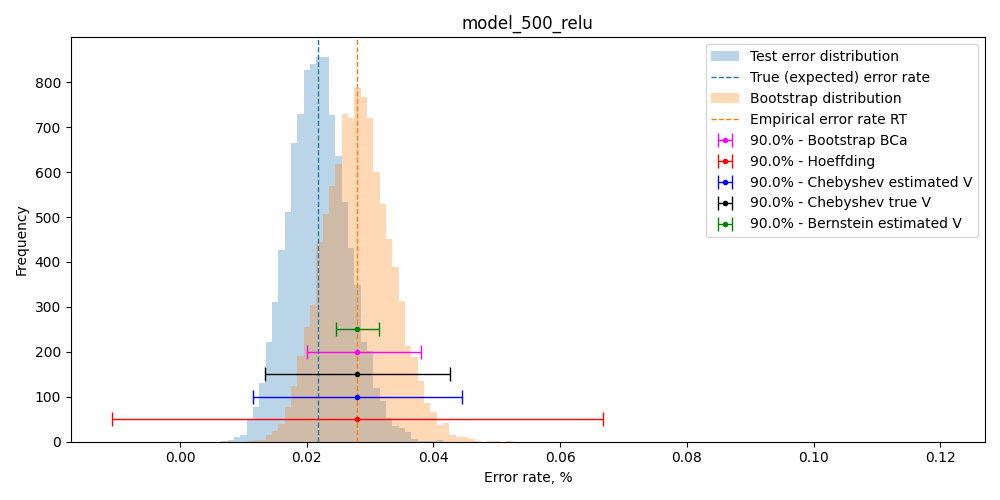
\includegraphics[width=\textwidth]{../errors/model_500_relu.png}
    \end{subfigure}
\end{figure}

\begin{table}[ht]
    \centering
    \begin{tabular}{ r | r | c | c | c | c }
        activation    & hidden & Hoeffding          & Chebyshev (estimated V) & Chebyshev (true V) & Bernstein          \\
        \hline
        \textit{tanh} & 5      & $0.042 \pm 0.0387$ & $0.042 \pm 0.0201$      & $0.042 \pm 0.0194$ & $0.042 \pm 0.0043$ \\
        \textit{ReLU} & 5      & $0.175 \pm 0.0387$ & $0.175 \pm 0.0380$      & $0.175 \pm 0.0397$ & $0.175 \pm 0.0122$ \\
        \textit{tanh} & 100    & $0.033 \pm 0.0387$ & $0.033 \pm 0.0179$      & $0.033 \pm 0.0184$ & $0.033 \pm 0.0037$ \\
        \textit{ReLU} & 100    & $0.025 \pm 0.0387$ & $0.025 \pm 0.0156$      & $0.025 \pm 0.0169$ & $0.025 \pm 0.0031$ \\
        \textit{tanh} & 500    & $0.037 \pm 0.0387$ & $0.037 \pm 0.0189$      & $0.037 \pm 0.0167$ & $0.037 \pm 0.0039$ \\
        \textit{ReLU} & 500    & $0.028 \pm 0.0387$ & $0.028 \pm 0.0165$      & $0.028 \pm 0.0146$ & $0.028 \pm 0.0033$ \\
    \end{tabular}
\end{table}

From the plots and the table we can spot a interesting behaviour with the $ReLU$ activation and $5$ hidden units.
The bootstrap distribution is completely off the (empirically computed) true error distribution.
But as we have seen in the previous task, this case behaved weirdly even regarding the decision boundary, which was almost linear, so perhaps it is not that suspicious.
\end{document}
